\documentclass[a4paper,10pt]{article}
\usepackage[utf8x]{inputenc}
\usepackage[utf8x]{inputenc}
\usepackage[OT1]{fontenc}
\usepackage{hyperref}
\usepackage{Sweave}
\usepackage{graphicx}
\usepackage{color}
\graphicspath{figures/}
\usepackage{float}
\usepackage{wrapfig}
\usepackage{subfigure}
%% Package to linebreak URLs in a sane manner.
\usepackage{url}
%% Define a new 'smallurl' style for the package that will use a smaller font.
\makeatletter
\def\url@smallurlstyle{%
  \@ifundefined{selectfont}{\def\UrlFont{\sf}}{\def\UrlFont{\small\ttfamily}}}
\makeatother
%% Now actually use the newly defined style.
\urlstyle{smallurl}
%% Define 'tinyurl' style for even smaller URLs (such as in tables)
\makeatletter
\def\url@tinyurlstyle{%
  \@ifundefined{selectfont}{\def\UrlFont{\sf}}{\def\UrlFont{\scriptsize\ttfamily}}}
\makeatother
%% Make margins less ridiculous
\usepackage{fullpage}
%% Make URLs clickable
%\usepackage[colorlinks, bookmarks=false]{hyperref}
%\usepackage[colorlinks, bookmarks=true]{hyperref}
%% Since I'm using the LaTeX Makefile that uses dvips, I need this
%% package to make URLs break nicely
\usepackage{breakurl}
\usepackage{todonotes}
\usepackage{amsmath,amsfonts}
\numberwithin{equation}{subsection}
%%\usepackage{nonfloat}
\usepackage{bbm}
\usepackage{setspace}
\onehalfspacing
\usepackage{tabularx}

%
%
%
\usepackage{listings}
\usepackage{courier}
\lstset{
         basicstyle=\footnotesize\ttfamily, % Standardschrift
         %numbers=left,               % Ort der Zeilennummern
         numberstyle=\tiny,          % Stil der Zeilennummern
         stepnumber=2,               % Abstand zwischen den Zeilennummern
         numbersep=5pt,              % Abstand der Nummern zum Text
         tabsize=2,                  % Groesse von Tabs
         extendedchars=true,         %
         breaklines=true,            % Zeilen werden Umgebrochen
         keywordstyle=\color{red},
    		frame=b,         
 %        keywordstyle=[1]\textbf,    % Stil der Keywords
 %        keywordstyle=[2]\textbf,    %
 %        keywordstyle=[3]\textbf,    %
 %        keywordstyle=[4]\textbf,   \sqrt{\sqrt{}} %
         stringstyle=\color{white}\ttfamily, % Farbe der String
         showspaces=false,           % Leerzeichen anzeigen ?
         showtabs=false,             % Tabs anzeigen ?
         xleftmargin=17pt,
         framexleftmargin=18pt,
         framexrightmargin=6pt,
         framexbottommargin=4pt,
         %backgroundcolor=\color{lightgray},
         showstringspaces=false      % Leerzeichen in Strings anzeigen ?        
 }
 \lstloadlanguages{% Check Dokumentation for further languages ...
         %[Visual]Basic
         %Pascal
         %C
         %C++
         %XML
         %HTML
         %Java
 }
%\DeclareCaptionFont{blue}{\color{blue}} 
%\captionsetup[lstlisting]{singlelinecheck=false, labelfont={blue}, textfont={blue}}
\usepackage{caption}
\DeclareCaptionFont{white}{\color{white}}
\DeclareCaptionFormat{listing}{\colorbox[cmyk]{0.20, 0.20, 0.20, 0.01}{\parbox{0.98\textwidth}{\hspace{15pt}#1#2#3}}}
\captionsetup[lstlisting]{format=listing,labelfont=white,textfont=white, singlelinecheck=false, margin=0pt, font={bf,footnotesize}}
%
%

%opening
\title{Sanity check and the Trajectory workflow test}
\author{Pavel Senin}

\begin{document}

\maketitle

\begin{abstract}
This document has dual purpose. First of all, by writing it I am following the common Trajectroy analysis workflow reviewing 
all steps and debugging for errors. The second purpose is to compile a primer of Trajectory-aided SCM data mining.
\end{abstract}

\section{Outline}
At the beginning I will discuss the research question.

First section \ref{sec:first} explains the data aggregation within the Trajectory DB. I discuss two issues: first is
the data organization and its curation through preliminary analysis. Second issue is the pre-aggregation of data by 
time intervals (chunks) for future indexing.

In the second section \ref{sec:second} I address the Symbolic aggregation workflow. I cover the data specificity,
SAX parameters section and the index organization.

In the third section \ref{sec:third} I address the mining question.

\section{Research question}
The research question I am trying to resolve with this work is the discovery of recurrent behaviors within the Android SCM
trails by SAX application. Previously a variety of time-series mining algorithms was applied to the problem of finding
of periodicity and \textbf{recurrent behaviors} within the \textbf{software change artifacts trails} such as Linear predictive
coding and cepstrum coefficients \cite{citeulike:3378725}, Fourier Transform \cite{citeulike:10377345}
and coding \cite{citeulike:10377366}. Two last cited papers show that corresponding techniques allow the discovery of the 
strong signal corresponding to the release of MySQL.
Lin\&Keogh \cite{citeulike:2821475} discovered and explored universal application power 
of Symbolic Aggregate Approximation to variety of time-series data. 

In this work I explore the application of the SAX to the problem of discovering recurrent behaviors from software change 
artifacts trails.

To be precise in this writing I will check if I can see that there is a difference in recurrent behaviours before and after 
software release.

\subsection{Definitions}
Let's define 
\begin{itemize}
 \item the \textbf{sub-series of the \textit{length $W$, $S_{W}$}} as the 
    continous interval extracted from the larger time-series, analogous to sub-string;
 \item the \textbf{SAX representation of sub-series $S_{W}$ by \textit{PAA of size $P$} and 
    an \textit{Alphabet of size $A$}} as the symbolic representation of the 
    sub-series $S_{W}$ obtained by PAA and SAX transforms.
\end{itemize}

For example, consider the sub-series of size 7 from time-series of daily commits $S_{7}$ by some contributor: $\{0,5,2,3,4,3,0\}$.
The contributor committed zero times at Sunday, five times Monday and so on. By applying PAA transform of length $3$ and SAX 
transform with the Normal alphabet of size $3$ we will get a $P_{3}A_{3}$ representation of $S_{7}$ which will be $bbb$. 
Note how choice of the week format (starting from Sunday or Monday) affects the result. If we will do the same transform for 
$\{5,2,3,4,3,0,0\}$ the result will be $cca$\ldots

\subsection{Methodology}
I define series and events of interest. 
By applying the transform defined by $W$ - sliding window size, $P$ - paa length and $A$ - alphabet size I extract all possible
strings from all of the series of interest. 
By comparing and mining of these dictionaries I will discover recurrent behaviors.

\subsection{Behaviors taxonomy}
I propose to use and will explore the application of \textit{``busy weekend''} pattern,
\textit{``consistent development''} and \textit{``sporadic development''} patterns, 
and a \textit{``long night''} pattern for the discovery of a software release. 


\section{Aggregating commits statistics in TrajectoryDB}\label{sec:first}
The raw statistics from an SCM system is stored within the TajectoryDB. There is information about every change, its impact
on the source code tree and an auxiliary data about projects and contributors.

For the first test I have randomly selected a contributor with id \emph{153} (davem$@$davemloft.net) and a project with id 
\emph{18} (android-kernel-omap). 
As a daytime interval I have chosen the \emph{nt} interval corresponding to night hours from \emph{5PM to 00AM}. 
Let's the see records in the change database first by querying it with the query from listing \ref{query1}:

\noindent\begin{minipage}{\textwidth}
\begin{lstlisting}[label=query1,caption=Data summary retrieval SQL query]
select c.id, c.author_date, c.subject, sum(c.added_files) ta, 
 sum(c.edited_files) te, sum(c.removed_files) td, sum(c.added_lines) la, 
 sum(c.edited_lines) le, sum(c.removed_lines) ld from android_change c 
 where c.author_id=153 and c.project_id=18 
 AND c.author_date between "2010-03-01" AND "2010-04-01"
 and date_format(c.author_date,'%H') between 17 and 23
 group by c.id order by c.author_date;
\end{lstlisting}
\end{minipage}
\begin{table}[hb]
\noindent\begin{minipage}{\textwidth}
  \tiny
  \caption{Result of running the query \ref{query1} against the TrajectoryDB (the column names are truncated for illustration purposes). }
  \begin{tabularx}{\textwidth}{ | l | l | X | r | r | r | r | r | r | r |}
  \hline           
id & author\_date & subj & ta & te & td & la & le & ld\\ 
\hline           
827962 & 2010-03-03 17:08 & \verb7sparc64: Kill off old sys_perfctr system call and state.7 & 0 & 12 & 0 & 0 & 18 & 195\\ 
827955 & 2010-03-03 18:06 & \verb1sparc64: Make prom entry spinlock NMI safe.1 & 0 & 1 & 0 & 0 & 7 & 0\\ 
827241 & 2010-03-05 22:41 & \verb1timbgpio: fix build1 & 0 & 1 & 0 & 1 & 0 & 0\\ 
826446 & 2010-03-10 22:05 & \verb1uartlite: Fix build on sparc.1 & 0 & 1 & 0 & 0 & 5 & 0\\ 
825982 & 2010-03-13 21:17 & \verb1Merge branch 'master' of1 & 0 & 0 & 0 & 0 & 0 & 0\\
& & \verb1git://git.kernel.org/pub/scm/linux/kernel/git/linville/wireless-2.61 &  &  &  &  &  & \\  
825784 & 2010-03-15 23:23 & \verb7e100: Fix ring parameter change handling regression.7 & 0 & 1 & 0 & 0 & 1 & 0\\ 
825679 & 2010-03-16 22:37 & \verb1bridge: Make first arg to deliver_clone const.1 & 0 & 1 & 0 & 0 & 4 & 0\\ 
825678 & 2010-03-16 22:40 & \verb7sunxvr1000: Add missing FB=y depenency.7 & 0 & 1 & 0 & 0 & 1 & 0\\ 
825288 & 2010-03-20 22:41 & \verb1Merge branch 'vhost' of 1 & 0 & 0 & 0 & 0 & 0 & 0\\
& & \verb1git://git.kernel.org/pub/scm/linux/kernel/git/mst/vhost1 &  &  &  &  &  & \\  
825287 & 2010-03-20 23:24 & \verb1Merge branch 'master' of 1 & 0 & 0 & 0 & 0 & 0 & 0\\ 
& & \verb1master.kernel.org:/pub/scm/linux/kernel/git/davem/net-2.61 &  &  &  &  &  & \\  
824847 & 2010-03-25 19:48 & \verb1Merge branch 'master' of 1 & 0 & 0 & 0 & 0 & 0 & 0\\ 
& & \verb1git://git.kernel.org/pub/scm/linux/kernel/git/kaber/nf-2.61 &  &  &  &  &  & \\  
824789 & 2010-03-26 18:23 & \verb7Revert r8169: enable 64-bit DMA by default for PCI Express devices (v2)"7 & 0 & 1 & 0 & 4 & 3 & 8\\ 
824627 & 2010-03-29 22:08 & \verb1sparc64: Properly truncate pt_regs framepointer in perf callback.1 & 0 & 1 & 0 & 0 & 1 & 0\\ 
824620 & 2010-03-29 22:50 & \verb9Merge branch 'master' of 9 & 0 & 0 & 0 & 0 & 0 & 0\\
& & \verb+git://git.kernel.org/pub/scm/linux/kernel/git/linville/wireless-next-2.6+ &  &  &  &  &  & \\  
\hline           
  \end{tabularx}
\end{minipage}
  \label{tab:origins}
\end{table}

Here five of fourteen commits: \emph{825982, 825288, 825287, 824847, 824620} are in fact merge commits. For these
I am unable to collect any of the statistics. Thus there is a question - \textit{should I count these merege commits 
(which have zero statistics) as an activity or should I skip commits which have
zero changes attached?} I think I should include these into analyses since even if the change appears to be empty
it anyway requires some of the developer's attention to actually make a merge decision, to perform the merge, 
and to check its results. I double-checked the information of MSR XML file and my pipeline by checking out OMAP 
repository locally and traversing 
the tree, see Figure \ref{fig:git_screen}. It seems to be that Git doesn't have any data about the merge. 
Maybe it can be recalled by traversing the tree up or down, but this is not implemented.

\begin{figure}[h]
   \centering
   \includegraphics[width=\textwidth]{figures/Screenshot-gitk:omap.ps}
   \caption{The GUI git viewer screenshoot illustrating commit statistics.}
   \label{fig:git_screen}
\end{figure}

It is nice to see that TrajectoryDB has all the data immediately available in Git, however the result in the Table 
\ref{tab:origins} is not very suitable for further analyses because changes retrieved are sequential. I decided to
use MySQL functions to aggregate data. The query used within the trajectory workflow shown at the listing 
\ref{query2}.

\noindent\begin{minipage}{\textwidth}
\begin{lstlisting}[label=query2,caption=Data summary retrieval SQL query with aggergation by date]
select date_format(c.author_date, '%Y-%m-%d') as day, count(distinct(c.id)) as commits, 
 sum(c.added_files) as added_files, sum(c.edited_files) as edited_files, sum(c.removed_files) as removed_files, 
 sum(c.added_lines) as added_lines, sum(c.edited_lines) as edited_lines, sum(c.removed_lines) as removed_lines 
 FROM android_change c 
 where c.author_id=153 and c.project_id=18 
 and c.author_date between "2010-03-01" AND "2010-04-01"
 and date_format(c.author_date,'%H') between 17 and 23 
 group by date_format(c.author_date, '%Y%m%d');
\end{lstlisting}
\end{minipage}

\begin{table}[hb]
\noindent\begin{minipage}{\textwidth}
  \caption{Result of running the query from Listing \ref{query2} against the TrajectoryDB.}
  \begin{tabularx}{\textwidth}{ | X | r | r | r | r | r | r | r | }
  \hline           
day & commits & added\_fs & edited\_fs & rm\_fs & added\_ls & edited\_ls & rm\_ls\\ 
\hline           
2010-03-03 & 2 & 0 & 13 & 0 & 0 & 25 & 195\\ 
2010-03-05 & 1 & 0 & 1 & 0 & 1 & 0 & 0\\ 
2010-03-10 & 1 & 0 & 1 & 0 & 0 & 5 & 0\\ 
2010-03-13 & 1 & 0 & 0 & 0 & 0 & 0 & 0\\ 
2010-03-15 & 1 & 0 & 1 & 0 & 0 & 1 & 0\\ 
2010-03-16 & 2 & 0 & 2 & 0 & 0 & 5 & 0\\ 
2010-03-20 & 2 & 0 & 0 & 0 & 0 & 0 & 0\\ 
2010-03-25 & 1 & 0 & 0 & 0 & 0 & 0 & 0\\ 
2010-03-26 & 1 & 0 & 1 & 0 & 4 & 3 & 8\\ 
2010-03-29 & 2 & 0 & 1 & 0 & 0 & 1 & 0\\
\hline    
  \end{tabularx}
\end{minipage}
  \label{tab:second}
\end{table}

This looks much better - for every day I have aggregated data about number commits, added, edited, deleted files (\emph{added\_fs, edited\_fs, rm\_fs}),
and lines (\emph{added\_ls, edited\_ls, rm\_ls}).

This data is digested within the Trajectory further - I save it the table \emph{time\_patterns} which keeps aggregated data along with the daytime tags
and labels. This auxiliary information is being used for indexing and data mining in order to reduce the size of stored data and improve turn-around
time of workflow. Here I use the \emph{nt} tag for the ``night commits'', 5PM-12AM. By running the \emph{SELECT} query from Listing \ref{query3} I am 
verifying that data is stored as it was - without any modification.
\noindent\begin{minipage}{\textwidth}
\begin{lstlisting}[label=query3,caption=Data summary from time\_patterns table]
SELECT * FROM time_patterns WHERE project_id = 18
AND author_id=148 AND UPPER(dtag)=UPPER("NT")
AND day between "2010-03-01" AND "2010-04-01"
ORDER BY day ASC;
\end{lstlisting}
\end{minipage}
\begin{table}[h]
\noindent\begin{minipage}{\textwidth}
  \centering
  \caption{Result of running the SELECT query from Listing \ref{query3} against the TrajectoryDB.}
  \begin{tabularx}{0.8\textwidth}{ | X | r | r | r | r | r | r | r | r |}
  \hline           
day & dtag & commits & t\_ad & t\_ed & t\_dlt & l\_ad & l\_ed & l\_dlt\\ 
\hline           
2010-03-03 & nt & 2 & 0 & 13 & 0 & 0 & 25 & 195\\ 
2010-03-05 & nt & 1 & 0 & 1 & 0 & 1 & 0 & 0\\ 
2010-03-10 & nt & 1 & 0 & 1 & 0 & 0 & 5 & 0\\ 
2010-03-13 & nt & 1 & 0 & 0 & 0 & 0 & 0 & 0\\ 
2010-03-15 & nt & 1 & 0 & 1 & 0 & 0 & 1 & 0\\ 
2010-03-16 & nt & 2 & 0 & 2 & 0 & 0 & 5 & 0\\ 
2010-03-20 & nt & 2 & 0 & 0 & 0 & 0 & 0 & 0\\ 
2010-03-25 & nt & 1 & 0 & 0 & 0 & 0 & 0 & 0\\ 
2010-03-26 & nt & 1 & 0 & 1 & 0 & 4 & 3 & 8\\ 
2010-03-29 & nt & 2 & 0 & 1 & 0 & 0 & 1 & 0\\
\hline    
  \end{tabularx}
  \label{prestrings}
\end{minipage}
\end{table}

The repository trail data stored in this fashion considerably save the computation time. Running aggregation by time slot 
and summarizing changes as in query from Listing \ref{query2} could take a very long time over large repositories, whether running 
single \emph{SELECT} over indexed by user, project, dtag and day \emph{time\_patterns} table takes a fraction of a second.

\section{Indexing aggregated commits statistics with SAX}\label{sec:second}
This step is essential for the reduction of the data complexity and for enabling of the data mining. The SCM trails data 
is getting transformed into sub-series chunks at first. These sub-series are converted into the symbolic representation
and indexed at the next step.

\subsection{Data distribution}
Before explaining the Trajectory workflow with symbolic approximation and indexing, I would like to double-check some SAX 
preliminaries.
First of all, when defining SAX alphabets, Lin\&Keogh \cite{citeulike:2821475} assumed that the normalized series are 
following Gaussian (normal) distribution. Within their work they concluded that the most of the real-life timeseries 
(\textit{``large family of the time series data in our disposal''}) are approximately normally distributed, which, 
unfortunately, is not the case of the Android SCM data in my disposal. 
I have tested the distribution of values from OMAP data. It does not follow the Normal distribution, see \ref{fig:qqplots},
thus I assume that the efficiency of SAX approximation will deteriorate. At this point I am unable to estimate to which
degree it may happen since there is no relevant research I know about.
However, according to Lin\&Keogh, the correctness of the SAX algorithm is unaffected by distribution.
The lower-bounding property of the SAX distance measure guarantees correctness of results.

\begin{figure}[p]
   \centering
   \includegraphics[width=\textwidth]{figures/OMAP_qqplots.ps}
   \caption{The distribution of time-series values after normalization. OMAP-kernel.}
   \label{fig:qqplots}
\end{figure}

\subsection{Symbolic approximation}
\begin{wrapfigure}{}{0.42\textwidth}
  \begin{center}
     \caption{Result of the conversion of data from \ref{prestrings} into SAX strings.}
     \begin{tabularx}{0.4\textwidth}{ | X | r | r |}
      \hline           
       string\_id & string & date\\ 
      \hline    
      72 & cba & 2010-03-01\\ 
      65 & bab & 2010-03-03\\ 
      66 & bbb & 2010-03-05\\ 
      59 & abb & 2010-03-06\\ 
      66 & bbb & 2010-03-07\\ 
      67 & bbc & 2010-03-09\\ 
      60 & abc & 2010-03-10\\ 
      63 & bcb & 2010-03-11\\ 
      62 & bca & 2010-03-12\\ 
      66 & bbb & 2010-03-13\\ 
      70 & cab & 2010-03-14\\ 
      \ldots & \ldots & \ldots \\ 
      66 & bbb & 2010-03-30\\ 
      63 & bcb & 2010-03-31\\ 
      66 & bbb & 2010-04-01\\
      \hline    
     \end{tabularx}
     \label{tab:strings}
  \end{center}
\end{wrapfigure}

The data from the Table \ref{prestrings} is converted into SAX series on the next step. This process consists of 
five consecutive steps:

\begin{enumerate}
 \item Three parameters are selected: the sliding window size $W$, the PAA size $P$ and the alphabet size $A$. These parameters I store as the 
characteristic tag of the timeseries in form $WxPxAx$ where $x$ is the corresponding parameter value.
 \item By using sliding window, timeseries is chopped by sub-series each of which has the length of $W$. 
       There will be $L_{series} - W$ of such sub-series (I use $L$ as an abbreviation of length).
 \item Each of the sub-series is getting \href{''http://code.google.com/p/jmotif/wiki/ZNormalization''}{''normalized by energy''}.
       The purpose of this step is to equal all the sub-fragments by amplitude but preserve their shape configuration.
 \item Each of the normalized pieces is approximated by use of 
   \href{''http://code.google.com/p/jmotif/wiki/PAAapproximation''}{''\emph{P}iecewise \emph{A}ggregate \emph{A}pproximation''}.
   It works by slicing original time-series into $P$ pieces and computing and assigning values for these slices 
   (mean of all points within the piece). 
 \item Real-valued PAA series is converted into the string by using \href{http://code.google.com/p/jmotif/wiki/SAX}{SAX}.
       These strings will consist only of letters of pre-selected alphabet.
\end{enumerate}

The Figure \ref{tab:strings} illustrates the conversion of the discussed here data into symbolic result. 
This result are also shown at the Figure \ref{fig:march_patterns}. Figure \ref{fig:march_patterns2} displays the picture
of overall nightly commit trail for the user \#\emph{153} (davem$@$davemloft.net) and a project \#\emph{18} (android-kernel-omap).
\begin{figure}[h]
\noindent\begin{minipage}{\textwidth}
  \centering
  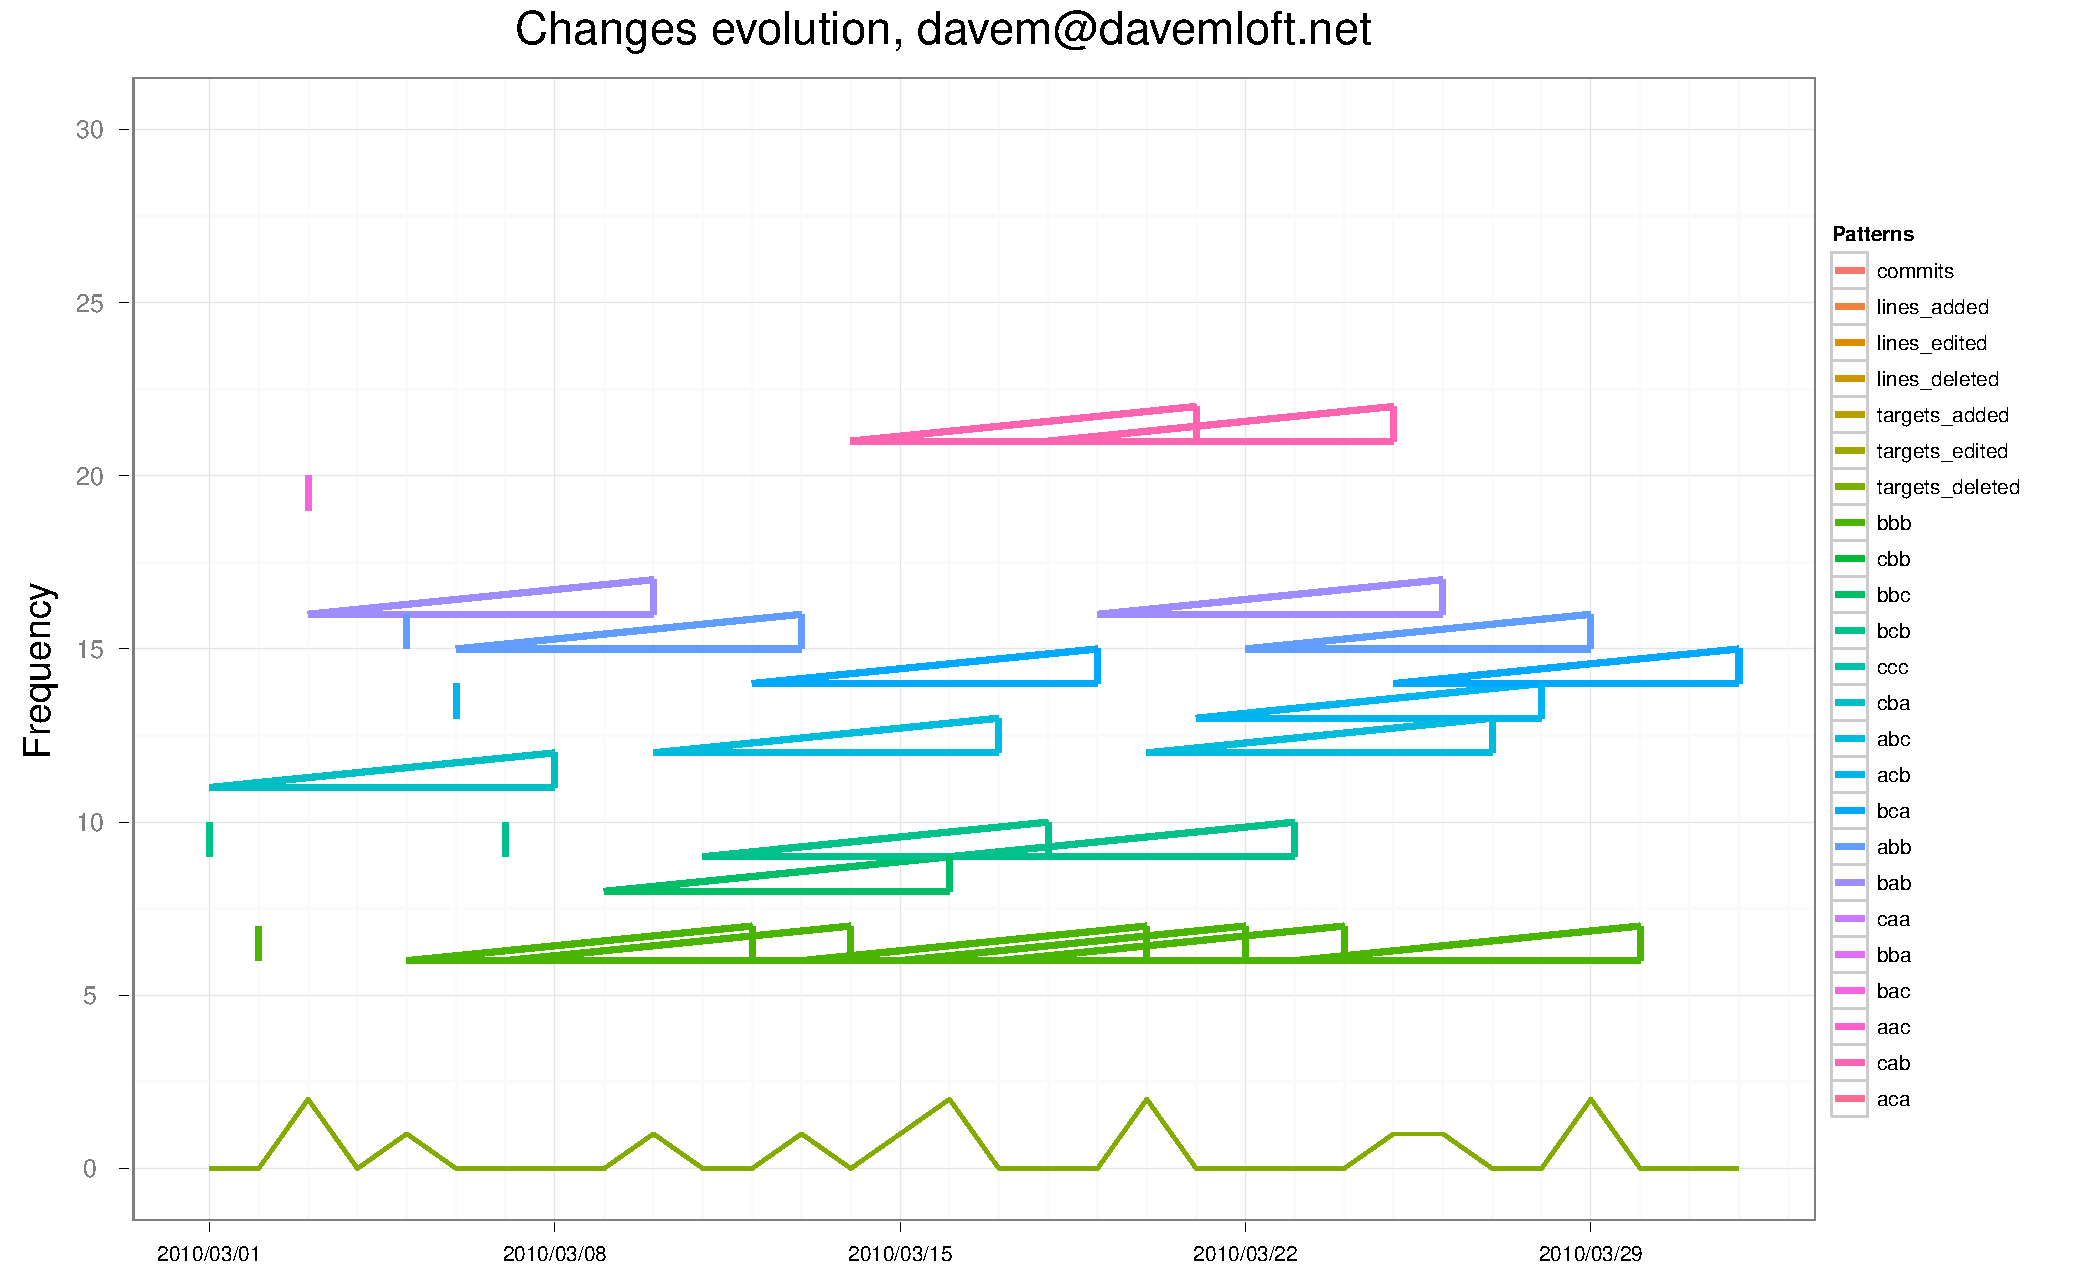
\includegraphics[width=\textwidth]{figures/march_fragment.ps}
  \caption{The illustration of the temporal distribution of patterns from Figure \ref{tab:strings}. Here I superimpose patterns over the 
commit frequency plot by using colored triangles. The curve at the very bottom is the commits frequency curve. Triangles representing 
patterns are  placed by the leftmost corner the pattern occurence start. The triangle length corresponds to the sliding window size -
 seven days, the color used for a triangle corresponds to the symbolic pattern. The small vertical lines at left are the right-side 
artifacts of patterns which do not fit into the current viewport (from 2010-03-01 to 2010-04-01)}
  \label{fig:march_patterns}
\end{minipage}
\end{figure}

\begin{figure}[h]
\noindent\begin{minipage}{\textwidth}
  \centering
  \includegraphics[width=\textwidth]{figures/long_patterns.ps}
  \caption{The illustration of the temporal SAX patterns distribution at the larger scale.}
  \label{fig:march_patterns2}
\end{minipage}
\end{figure}

\subsection{Choice of SAX parameters}
The cornerstone question in SAX transformation is the choice of the parameters. By varying the sliding window 
length I am able to slice the search space to only see patterns within the time-interval which is the length
of this window or it's miltiple (I need citation here about the choice of natural to data intervals)\ldots

For this time I picked weekly, bi-weekly and a monthly intervals. In my opinion they correspond to natural 
units of time within the software process. 

The choice of PAA size and an alphabet has a direct impact on the sensitivity of SAX algorithm and
on the size of the resulting dictionaries.
By varying the PAA size algorithm is able to smooth the high-frequency noise within the sliding window interval 
by aggregating values within the PAA piece to their mean value. By proper choice of PAA size it is possible to 
focus only on the certain-scale frequency within the data stream by analogy to FFT. The PAA size defines the length
of the resulting dictionary words. 
The choice of the alphabet size not only limits the amount of letters within the resulting words, thus having 
direct influence on the size and complexity of the dictionary, but tunes the sensityvity of the search.


to this length discriminate only this 

\begin{figure}[p]
   \centering
   \includegraphics[width=\textwidth]{figures/OMAP_qqplots.ps}
   \caption{The distribution of time-series values after normalization. OMAP-kernel.}
   \label{fig:qqplots}
\end{figure}


\subsection{Choice of storage strategy}


\section{Data Mining}\label{sec:third}
Here I discuss the results 

\subsection{Patterns classification}

\subsection{Hierarchical clustering}

\subsection{K-means clustering}

\section{Note to myself: wrong counts}
\noindent\begin{minipage}{\textwidth}
\begin{lstlisting}[label=query_wrong,caption=Wrong counts here in that second query due to the join. Look at the counts in third query to understand why]
select date_format(c.author_date, '%Y-%m-%d') as day, count(distinct(c.id)) as commits, 
sum(c.added_files) as added_files, sum(c.edited_files) as edited_files, 
sum(c.removed_files) as removed_files, sum(c.added_lines) as added_lines, 
sum(c.edited_lines) as edited_lines, sum(c.removed_lines) as removed_lines 
FROM android_change c 
where c.author_id=153 and c.project_id=18 
and c.author_date between "2010-03-01" AND "2010-04-01"
 and date_format(c.author_date,'%H') between 17 and 23 
group by date_format(c.author_date, '%Y%m%d');

select date_format(c.author_date, '%Y-%m-%d') as day, count(distinct(c.id)) as commits, 
count(t.change_id) as t, sum(c.added_files) as added_files, sum(c.edited_files) 
as edited_files, sum(c.removed_files) as removed_files, sum(c.added_lines) as added_lines, 
sum(c.edited_lines) as edited_lines, sum(c.removed_lines) as removed_lines 
FROM android_change c 
left join change_target t on c.id=t.change_id
where c.author_id=153 and c.project_id=18 
and c.author_date between "2010-03-01" AND "2010-04-01"
 and date_format(c.author_date,'%H') between 17 and 23 
group by date_format(c.author_date, '%Y%m%d');

select c.*, t.*
FROM android_change c 
left join change_target t on c.id=t.change_id
where c.author_id=153 and c.project_id=18 
and c.author_date between "2010-03-01" AND "2010-04-01"
 and date_format(c.author_date,'%H') between 17 and 23;
\end{lstlisting}
\end{minipage}

\bibliographystyle{abbrv}
\bibliography{seninp}

\end{document}
